% vim: ts=2 sts=2 sw=2

\documentclass[a4paper,12pt]{report}
\usepackage{a4wide}
\usepackage[finnish]{babel}
\usepackage[utf8]{inputenc}
\usepackage[T1]{fontenc}
\usepackage{graphicx}
\usepackage{float}

\title{
\includegraphics[width=5em]{logo}\\\vspace{1em}MusicGhost\\\vspace{1em}
  \large{Tietokantasovellus, kevät 2011\\Tietojenkäsittelytieteen
  laitos\\Helsingin yliopisto}\\}
\author{Tuomo Lempiäinen\\\texttt{tuomo.lempiainen@helsinki.fi} \and
Hanna Nieminen\\\texttt{hanna.m.nieminen@helsinki.fi}}

\begin{document}

\maketitle

\tableofcontents

\chapter{Määrittely}

\section{Johdanto}

\subsection{Järjestelmän tarkoitus}

Järjestelmän avulla sen ylläpitäjä voi pitää kirjaa levykokoelmastaan.
Järjestelmä tarjoaa useita erillisiä listoja, jolloin on mahdollista
erotella esimerkiksi omistamansa levyt ja tulevat hankinnat toisistaan.
Järjestelmästä voi tehdä julkisen, jolloin myös vierailijat voivat selata
levylistaa ja yksittäisten levyjen tietoja.

\subsection{Toimintaympäristö}

Järjestelmää käytetään WWW-selaimen kautta. Sen ajamiseen tarvitaan
Apache-palvelin varustettuna PHP5-tuella sekä PostgreSQL-tietokanta.

\subsection{Rajaukset}

Kaikki ominaisuudet, joita ei ole tässä määrittelyssä erikseen mainittu, on
oletusarvoisesti rajattu järjestelmän ulkopuolelle.

\subsection{Toteutusympäristö}

Järjestelmän toteuttamisessa hyödynnetään Vim-editoria Arch Linux
-käyttöjärjestelmässä sekä Notepad++-editoria Windows 7
-käyttöjärjestelmässä. Toteutuksen aikana järjestelmää testataan
paikallisilla Apache- ja PostgreSQL-palvelimilla.

\section{Yleiskuva järjestelmästä}

\subsection{Sidosryhmäkaavio}

\vspace{1em}
\begin{figure}[H]
  \begin{center}
    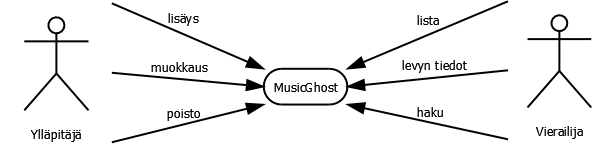
\includegraphics[width=\textwidth]{diagrams/sidosryhmakaavio}
  \end{center}
  \caption{Sidosryhmäkaavio}
\end{figure}

\subsection{Käyttäjäryhmät}

\begin{description}
  \item[Ylläpitäjä] Levytietokannan omistaja, joka ylläpitää tietokantaa.
  \item[Vierailija] Kuka tahansa sivulla vieraileva käyttäjä. Myös
    tietokannan omistaja kuuluu tähän luokkaan.
\end{description}

\section{Käyttötapaukset}

\subsection{Ylläpitäjä}

\begin{description}
  \item[Levyn lisääminen] Ylläpitäjä voi lisätä uusia levyjä tietokantaan.
    Ylläpitäjä syöttää ainakin levyn esittäjän, nimen, tyypin
    (albumi/single/\ldots) ja mahdollisen kokonaisuuden (boksin), johon levy
    kuuluu, sekä valitsee ainakin yhden listan, jolle se lisätään.
    Vapaaehtoisia tietoja ovat levyn julkaisuvuosi, formaatti, kotelointi,
    levy-yhtiö, painoksen koko, hankintapäivämäärä, tieto levyn lainassa
    olemisesta, vapaamuotoinen kommentti ja kansikuva.
  \item[Levyn tietojen muokkaaminen] Ylläpitäjä voi muokata kaikkia
    yksittäiseen levyyn liitettyjä tietoja.
  \item[Levyn poistaminen] Ylläpitäjä voi poistaa levyn tietokannasta.
  \item[Kirjautuminen ulos] Ylläpitäjä voi tarvittavat ylläpitotehtävät
    tehtyään kirjautua ulos, jolloin hänestä tulee tavallinen vierailija.
\end{description}

\subsection{Vierailija}

\begin{description}
  \item[Levylistan selaaminen] Kuka tahansa voi katsella tietokannan
    sisältöä.  Listauksessa näkyy kunkin levyn kohdalla sen esittäjä, nimi,
    julkaisuvuosi ja formaatti.
  \item[Yksittäisen levyn tietojen tutkiminen] Käyttäjä voi valita
    yksittäisen levyn, jolloin hänelle näytetään kaikki siihen liitetyt
    tiedot.
  \item[Levyjen hakeminen hakusanalla] Käyttäjä voi antaa hakusanoja,
    jolloin hänelle näytetään lista niistä levyistä, joiden listauksessa
    näytettävät tiedot sisältävät annetut hakusanat.
  \item[Kirjautuminen sisään] Mikäli vierailija tietää ylläpitäjän
    salasanan, hän voi kirjautua sisään järjestelmään, jolloin hänestä tulee
    ylläpitäjä.
\end{description}

\chapter{Suunnittelu}

\section{Järjestelmän tietosisältö}

\begin{figure}[H]
  \begin{center}
    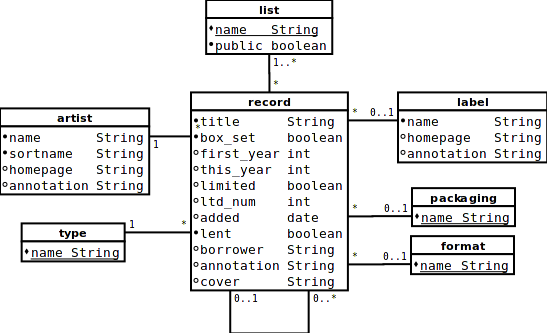
\includegraphics[width=0.8\textwidth]{diagrams/kasitekaavio}
  \end{center}
  \caption{Käsitekaavio}
\end{figure}

\begin{description}

  \item[artist]
    Levyn esittäjä identifioidaan yksikäsitteisen kokonaisluku-id:n avulla.
    Esittäjä voi liittyä tietokannassa mielivaltaiseen määrään levyjä.
    \begin{description}
      \item[name] Esittäjän nimi (esimerkiksi ''Etunimi Sukunimi'')
      \item[sortname] Nimi, jota käytetään esittäjien järjestämiseen
        (esimerkiksi ''Sukunimi, Etunimi'')
      \item[homepage] Esittäjän kotisivujen osoite
      \item[annotation] Vapaamuotoinen kuvaus esittäjästä
    \end{description}

  \item[label]
    Levy-yhtiö identifioidaan yksikäsitteisen kokonaisluku-id:n avulla.
    Levy-yhtiö voi liittyä tietokannassa mielivaltaiseen määrään levyjä.
    \begin{description}
      \item[name] Levy-yhtiön nimi
      \item[homepage] Levy-yhtiön kotisivujen osoite
      \item[annotation] Vapaamuotoinen kuvaus levy-yhtiöstä
    \end{description}

  \item[record]
    Omistajan levykokoelmaan kuuluva levy. Levy identifioidaan
    yksikäsitteisen kokonaisluku-id:n avulla.  Levyyn liittyy sen esittäjä
    ja tyyppi. Siihen voi liittyä myös enintään yksi levy-yhtiö, formaatti
    ja kotelon tyyppi.  Lisäksi levy kuuluu ainakin yhteen listaan. Levy voi
    kuulua samaan boksiin joidenkin muiden levyjen kanssa.
    \begin{description}
      \item[title] Levyn nimi (merkkijono)
      \item[box\_set] Onko kyseessä boksi, johon voi sisältyä muita levyjä?
        (totuusarvo)
      \item[first\_year] Levyn alkuperäinen julkaisuvuosi (kokonaisluku)
      \item[this\_year] Kokoelmassa olevan version julkaisuvuosi (kokonaisluku)
      \item[limited] Onko levy rajoitettua painosta? (totuusarvo)
      \item[ltd\_num] Rajoitetun painoksen painosmäärä (kokonaisluku)
      \item[added] Päivä, jolloin levy on lisätty kokoelmaan (päivämäärä)
      \item[lent] Onko levy lainassa? (totuusarvo)
      \item[borrower] Henkilö, jolle levy on lainattu (merkkijono)
      \item[annotation] Vapaamuotoinen kuvaus levystä (merkkijono)
      \item[cover] Levyn kansikuvan tiedostonnimi (merkkijono)
    \end{description}

  \item[type]
    Levytyyppi voi liittyä tietokannassa mielivaltaiseen määrään levyjä.
    \begin{description}
      \item[name] Levyn tyyppi, esimerkiksi ''Album'' tai ''Single''
        (merkkijono)
    \end{description}

  \item[format]
    Levyformaatti voi liittyä tietokannassa mielivaltaiseen määrään levyjä.
    \begin{description}
      \item[name] Levyn formaatti, esimerkiksi ''2CD'' tai ''DVD+CD''
        (merkkijono)
    \end{description}

  \item[packaging]
    Kotelotyyppi voi liittyä tietokannassa mielivaltaiseen määrään levyjä.
    \begin{description}
      \item[name] Levyn kotelon tyyppi, esimerkiksi ''Jewel case'' tai
        ''Digipak'' (merkkijono)
    \end{description}

  \item[list]
    Levylista, johon voi liittyä mielivaltainen määrä levyjä.
    Lista identifioidaan sen yksikäsitteisen nimen perusteella.
    \begin{description}
      \item[name] Listan nimi (merkkijono)
      \item[public] Onko lista julkinen? (totuusarvo)
      \item[default] Onko kyseeessä oletuslista, joita on vain yksi?
        (totuusarvo)
    \end{description}

\end{description}

\section{Käyttöliittymän hahmotelma}

\begin{figure}[H]
  \begin{center}
    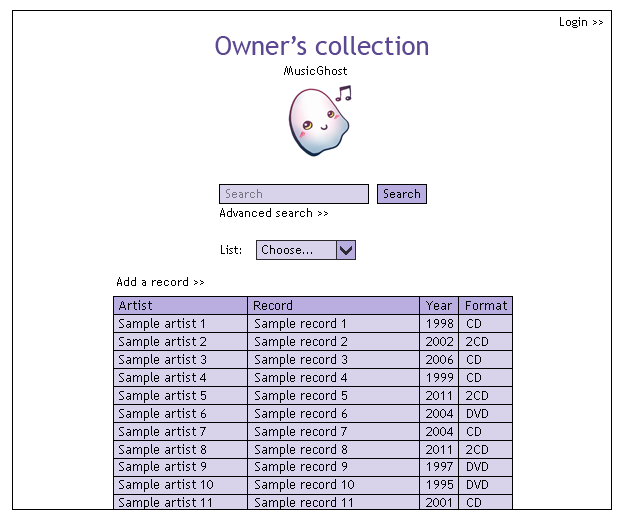
\includegraphics[width=\textwidth]{uidraft/mainwindow2}
  \end{center}
  \caption{Etusivu}
\end{figure}

\begin{figure}[H]
  \begin{center}
    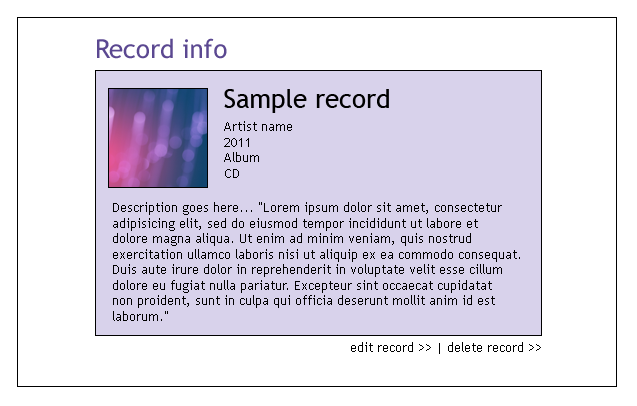
\includegraphics[width=\textwidth]{uidraft/recordinfopage}
  \end{center}
  \caption{Levyn lisätietosivu}
\end{figure}

\begin{figure}[H]
  \begin{center}
    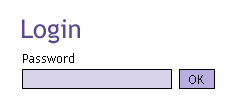
\includegraphics[]{uidraft/login}
  \end{center}
  \caption{Sisäänkirjautumissivu}
\end{figure}

\begin{figure}[H]
  \begin{center}
    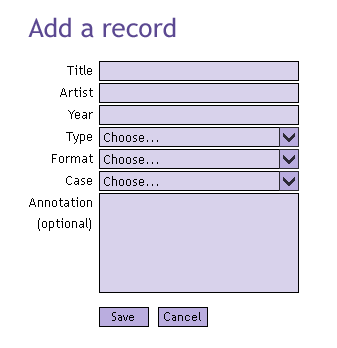
\includegraphics[]{uidraft/addpage}
  \end{center}
  \caption{Levyn lisäyssivu}
\end{figure}

\begin{figure}[H]
  \begin{center}
    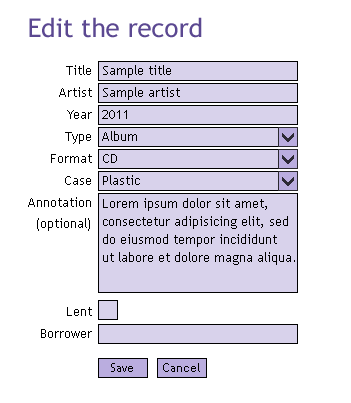
\includegraphics[]{uidraft/editpage}
  \end{center}
  \caption{Levyn muokkaussivu}
\end{figure}

\begin{figure}[H]
  \begin{center}
    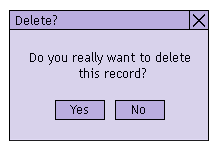
\includegraphics[]{uidraft/delete}
  \end{center}
  \caption{Levyn poiston varmistusdialogi}
\end{figure}

\section{Relaatiotietokantakaavio}

Relaatiotietokantakaavio on esitetty \texttt{CREATE TABLE} -lauseina
tiedostossa \texttt{sql/init\_db.sql}.

\end{document}
